\documentclass[../apprentice.tex]{subfiles}

\pagestyle{main}
\renewcommand{\chaptermark}[1]{\markboth{\chaptername\ \thechapter}{}}

\begin{document}




\chapter{}
\section{Gaussian Curvature (Neves)}
\begin{itemize}
    \item \marginnote{6/28:}Plan:
    \begin{enumerate}
        \item What is a surface?
        \item What is the tangent space?
        \item What are the principal curvatures?
        \item What is the Gaussian curvature?
    \end{enumerate}
    \item In analysis:
    \begin{enumerate}
        \item What is a function?
        \item What is the derivative?
        \item What is the Hemian of function?
        \item 2nd derivative test (determinant of Hemina).
    \end{enumerate}
    \item \textbf{Surface}: A subset $\sigma\subseteq\R^3$ such that for all $p\in\Sigma$, there's a neighborhood $B$ of $p$ in $\R^3$ so that $\Sigma\cap B$ "looks like a disk." More precisely, there exists an open neighborhood $U\subseteq\R^2$ and a map $\varphi:U\to\Sigma\cap B\subseteq\R^3$ such that
    \begin{enumerate}[label={\roman*)}]
        \item $\varphi$ is continuous and smooth.
        \item $\varphi$ is a bijection (with $\varphi^{-1}$ continuous).
        \item $\dd{\varphi}_{|x}:\R^2\to\R^3$ is injective for all $x\in U$.
    \end{enumerate}
    \item \textbf{Chart}: The quantity $(\varphi,U)$ near $p\in U$.
    \item Examples:
    \begin{enumerate}[label={\Alph*)}]
        \item Plane. $\Sigma=\R^2\times|0|\subseteq\R^3$ is a surface with chart $\varphi:\R^2\to\Sigma$ where $(x,y)\mapsto(x,y,0)$.
        \item Sphere. $\Sigma=\{\vec{u}\in\R^3\mid|\vec{u}|=1\}$.
        \begin{itemize}
            \item Charts: Consider the sets $U=\{(x_1,x_2)\mid {x_1}^2+{x_2}^2<1\}\subseteq\R^2$. Let $\varphi_1^+:U\to\Sigma\cap\{(x,y,z)\mid x>0\}$ be defined by $\varphi_1^+(u_1,u_2)=(\sqrt{1-{x_1}^2-{x_2}^2},u_1,u_2)$, $\varphi_1^-:U\to\Sigma\cap\{(x,y,z)\mid x<0\}$ be defined by $\varphi_1^-(u_1,u_2)=(-\sqrt{1-{x_1}^2-{x_2}^2},u_1,u_2)$.
            \item Same thing for $\varphi_2^\pm,\varphi_3^\pm$.
        \end{itemize}
        \item A cone $\Sigma=\{(x,y,z)\mid z=\sqrt{x^2+y^2}\}$ is \emph{not} a surface because it fails property (iii).
        \item The closed unit disk $\Sigma=\{(x,y,0)\mid x^2+y^2\leq 1\}$ is also not a surface.
    \end{enumerate}
    \item \textbf{Tangent space}: Let $\Sigma\subseteq\R^3$ be a surface and let $p\in\Sigma$. Then $T_p\Sigma\subseteq\R^3$ is the $z$-plane so that $p+T_p\Sigma$ is the affine plane that best approximates $\Sigma$ near $p$.
    \begin{itemize}
        \item Best linear approximation near the surface.
        \item Very similar/analogous to the derivative.
    \end{itemize}
    \item If $(\varphi,U)$ is a chart near $p$, then $T_p\Sigma=\text{span}\,\{\frac{\partial\varphi}{\partial x_1}(\bar{x}_1,\bar{x}_2),\frac{\partial\varphi}{\partial x_2}(\bar{x}_1,\bar{x}_2)\}$.
    \item Proves linear independence of above vectors.
    \item Principal curvatures.
    \item Let $\Sigma\subseteq\R^3$ be a surface, $p\in\Sigma$, and $\vec{N}$ be a unit normal vector defined around $p$ (i.e., $\vec{N}(q)\cdot\vec{v}=0$ for all $q$ near $p$ and $\vec{v}\in T_q\Sigma$).
    \item Choose $\vec{v}\in T_p\Sigma$ such that $|\vec{v}|=1$. Set $P_v=\text{span}\,\{\vec{v},\vec{N}(p)\}$. Claim: $(\Sigma-p)\cap P_v$ is a curve near the origin.
    \item \textbf{Principal curvature}: The reciprocal of the radius of the circle in $P_v$ that best approximates $(\Sigma-p)\cap P_v$ near the origin. \emph{Also known as} $\bm{K(\vec{v})}$.
    \begin{itemize}
        \item The sign is positive if the center of the circle is in the direction of $\vec{N}(p)$ and negative otherwise.
        \item If the sign of $\vec{N}(p)$ changes, then $K(\vec{v})$ will change in sign.
    \end{itemize}
    \item If we change $\vec{N}$ by $-\vec{N}$, then the new $K(\vec{v})$ is the opposite of the old one.
    \item Given $p\in\Sigma$ and $\vec{N}(p)$ a normal vector at $p$, we define $K_1(p)$ to have the maximum $K(\vec{v})$ over all unit vectors $\vec{v}\in T_p\Sigma$ and $K_2(p)=\min\{K(\vec{v})\mid \vec{v}\in T_p\Sigma,|\vec{v}|=1\}$.
    \item $K_1,K_2$ are computable quantities.
\end{itemize}



\section{Lecture 1.6: An Explicit Formula for the Catalan Numbers}
\begin{itemize}
    \item \marginnote{6/29:}Theorem (discovered by Euler):
    \begin{equation*}
        C_n = \frac{1}{n+1}\binom{2n}{n}=\frac{(2n)!}{n!(n+1)!}
    \end{equation*}
    \item Examples:
    \begin{itemize}
        \item $C_1=\frac{1}{2}\binom{2}{1}=1$.
        \item $C_2=\frac{1}{3}\binom{4}{2}=2$.
        \item $C_3=\frac{1}{4}\binom{6}{3}=5$.
    \end{itemize}
    \item Dyck path:
    \begin{itemize}
        \item We'll study paths starting with $(0,0)$, going on each stop either from $(x,y)$ to $(x+1,y+1)$ or from $(x,y)$ to $(x+1,y-1)$.
        \item Consider the number of ways to get to each point on the integer grid $\Z\times\Z$ from $(0,0)$.
        \begin{itemize}
            \item Generates a rotated Pascal's triangle.
            \item The number of paths from $(0,0)$ to $(a+b,a-b)$, i.e., $a$ moves up and $b$ moves down is $\binom{a+b}{b}$.
        \end{itemize}
    \end{itemize}
    \item Proposition: $C_n$ is equal to the number of paths from $(0,0)$ to $(2n,0)$ which are contained in the upper half-plane ($y\geq 0$).
    \begin{itemize}
        \item Proof: $C_n$ is the number of sequences of brackets.
        \item Transform a sequence of brackets into a path by $(\mapsto\nearrow$ and $)\mapsto\searrow$.
        \item The condition $\#(=\#)$ implies that the paths start at $(0,0)$ and end at $(2n,0)$.
        \item The condition that in every initial segment, $\#(=\#)$ implies that the path lies in the upper half plane.
    \end{itemize}
    \item Reflection principle:
    \begin{itemize}
        \item The number of paths from $A$ to $B$ in the upper half plane is equal to the number of paths from $A$ to $B$ minus the number of paths from $A$ to $B$ that intersect the line $y=-1$.
        \item Symbolically, $C_n=\binom{2n}{n}-$?
        \item There exists a one-to-one correspondence between two sets: The set of all paths from $A$ to $B$ intersecting $\ell$ and the set of all paths from $A$ to $B'$, where $B'$ is the reflection of $B$ across $\ell$.
    \end{itemize}
    \item Thus, the number of paths from $A$ to $B$ that intersect the line $y=-1$ is equal to the number of paths from $A$ to $(2n,-2)$.
    \item Therefore,
    \begin{align*}
        \binom{2n}{n}-\binom{2n}{n-1} &= \frac{(2n)!}{n!n!}\left( 1-\frac{n}{n+1} \right)\binom{2n}{n-1}\\
        &= \frac{1}{n+1}\binom{2n}{n}
    \end{align*}
    \begin{itemize}
        \item Note that it's not obvious that $\frac{1}{n+1}\binom{2n}{n}$ is an integer unless you present it as the difference of two binomials (i.e., as $\binom{2n}{n}-\binom{2n}{n-1}$).
    \end{itemize}
    \item Exercise:
    \begin{itemize}
        \item Take a path from $A$ to $B$ intersecting $\ell$ and find the closest point of $P\cap\ell$ to $B$. Reflect the segment of the path after this point.
    \end{itemize}
\end{itemize}



\section{Introduction to Quantitative Topology (Weinberger)}
\begin{itemize}
    \item \marginnote{7/1:}Topological Problems:
    \begin{itemize}
        \item Are $X$ and $Y$ homeomorphic?
        \item $f,g:X\to Y$. Does there exist a homotopy $f_t:X\to Y$, $f_0=f,f_1=g$?
        \item Given $X$, does it embed in $\R^n$?
    \end{itemize}
    \item When the answer is yes, something exists.
    \begin{itemize}
        \item But what can you tell me about the thing that exists?
        \item Typically, the adjective is, "how big?"
    \end{itemize}
    \item Suppose $M$ is an $n$-dimensional triangulated manifold, i.e., $\partial(\text{tetrahedron})=S^2$ (the boundary of $M$ is the two dimensional sphere).
    \item Poincar\'{e} conjecture: if $M$ looks like a sphere to an algebraic topologist, i.e.,
    \begin{itemize}
        \item $\pi_1(M)=e$.
        \item $\tilde{H}_i(M)=0$, $i<n$.
        \item $M$ is homotopy equivalent to $S^n$.
    \end{itemize}
    then it is a sphere, i.e., there exists some subdivision of $M$ and some subdivision of $\partial(\triangle^n)=S^n$ such that $M^\text{subdivided}$ and $(S^n)^\text{subdivided}$ are combinatorially isomorphic.
    \item How big means how many simplicities there are.
    \item Another quantitative question: Suppose I triangulate the sphere with $N$ simplicities. How much further subdivision do I need to do to make it a subdivision of the standard simplex.
    \item Consider $S^5$ (the 5-dimensional sphere).
    \begin{itemize}
        \item Consider $\N\mapsto f(\N)$, where $f(N)$ is the biggest number you need to be able to see $M\approx S^5$ combinatorially.
        \item Consider the number of protons in the universe. Is it 10, $\N$, $N^?$, $\log(N^2)$, $2^{2^{2^{\nearrow^N}}}$? It's none of the above; $>$ all of them.
    \end{itemize}
\end{itemize}



\section{PSet 2}
\begin{enumerate}
    \item \marginnote{6/30:}Consider $n$ pairs of points on the segment $AB$, which are symmetric with respect to its center. Half of these points are red, the other are blue. Prove that the sum of distances from the point $A$ to the blue points equals the sum of distances from the point $B$ to the red points.
    \begin{proof}
        Let $C$ be the midpoint of $AB$. Clearly, if every point is located at $C$, the sum of the distances from $A$ to the blue points is $n\cdot\text{len}\,(AC)$, and similarly for $B$ and the red points. Thus, to prove the claim, it will suffice to show that moving any pair of points located at $C$ to two points that are symmetric with respect to $C$ preserves the equality of the $A$-to-blue-points and $B$-to-red-points distances. We divide into three cases (both points are blue, both points are red, and one point is blue and the other red).\par
        If both points are blue, then moving them will not affect the $B$-to-red-points distance. As such, we must show that moving them symmetrically similarly does not affect the $A$-to-blue-points distance. But this is obviously true, as shortening the distance from $A$ to $p_1$ by $\ell$ necessitates lengthening the distance from $A$ to $p_2$ by $\ell$, cancelling out any potential change.\par
        The proof is symmetric if both points are red.\par
        If one point is blue and the other red, then shortening the distance from $A$ to $p_b$ by $\ell$ necessitates shortening the distance from $B$ to $p_r$ by $\ell$ as well, preserving equality. Vice versa is true for lengthening the distance from $A$ to $p_b$.
    \end{proof}
    \item Consider a set $2^S$ of subsets $S=\{1,2,\dots,n\}$. For two subsets $A,B\in 2^S$, define their symmetric difference by $A\triangle B=(A\cup B)\setminus(A\cap B)$. Prove that $2^S$ with this operation is a group.
    \begin{proof}
        To prove tht $2^S$ with $\triangle$ is a group, we must verify the associativity, identity, and inverse conditions.\par
        To confirm that $2^S$ is associative, we must show that for all $A,B,C\in G$, $(A\triangle B)\triangle C=A\triangle(B\triangle C)$. Let $A,B,C$ be arbitrary elements of $2^S$. Then
        \begin{align*}
            (A\triangle B)\triangle C &= ((A\cup B)\setminus(A\cap B))\triangle C\\
            &= (((A\cup B)\setminus(A\cap B))\cup C)\setminus(((A\cup B)\setminus(A\cap B))\cap C)\\
            % &= (((A\setminus B)\cup(B\setminus A))\cup C)\setminus(((A\setminus B)\cup(B\setminus A))\cap C)\\
            % &= (((A\setminus B)\cup(B\setminus A))\setminus C)\cup(((A\setminus B)\cup(B\setminus A))\setminus C)\\
            &= (A\cup((B\cup C)\setminus(B\cap C)))\setminus(A\cap((B\cup C)\setminus(B\cap C)))\\
            &= A\triangle((B\cup C)\setminus(B\cap C))\\
            &= A\triangle(B\triangle C)
        \end{align*}
        Note that the two big expressions are equal since we can show that they are both represented by the following picture, where the shaded area may have elements and the unshaded area cannot\footnote{Note that there is an alternate proof of this: Write each set as a permutation of 1s and 0s. Define a bijection $f$ with the property that $f(A\triangle B)=(f(A)+F(B))\text{mod}\,2$. Then commutativity follows easily.}.
        \begin{figure}[h!]
            \centering
            \begin{tikzpicture}
                \footnotesize
                \filldraw [rez] (90:1.15) arc (59:240:1cm) arc (178:118:1cm) arc (182:122:1cm);
                \filldraw [rez] (-30:1.15) arc (-61:120:1cm) arc (58:-2:1cm) arc (62:2:1cm);
                \filldraw [rez] (210:1.15) arc (179:360:1cm) arc (298:238:1cm) arc (302:242:1cm);
                \filldraw [rez] (30:0.55) arc (-2:-59:1cm) arc (-122:-178:1cm) arc (119:60:1cm);

                \draw (30:0.6) circle (1cm) node[right=4mm]{$B$};
                \draw (150:0.6) circle (1cm) node[left=4mm]{$A$};
                \draw (-90:0.6) circle (1cm) node[below=4mm]{$C$};
            \end{tikzpicture}
            \caption{Power set group associativity.}
            \label{fig:2S-associativity}
        \end{figure}\par
        To confirm that the identity element is the $\emptyset$, it will suffice to show that $A\triangle\emptyset=\emptyset\triangle A=A$ for all $A\in 2^S$. Let $A$ be an arbitrary element of $2^S$. Then
        \begin{align*}
            A\triangle\emptyset &= (A\cup\emptyset)\setminus(A\cap\emptyset)\\
            &= A\setminus\emptyset\\
            &= A\\
            &= A\setminus\emptyset\\
            &= (\emptyset\cup A)\setminus(\emptyset\cap A)\\
            &= \emptyset\triangle A
        \end{align*}
        as desired.\par
        To confirm $A=A^{-1}$, we must show that $A\triangle A=\emptyset$. But we have that
        \begin{align*}
            A\triangle A &= (A\cup A)\setminus(A\cap A)\\
            &= A\setminus A\\
            &= \emptyset
        \end{align*}
        as desired.
    \end{proof}
    \item Let $G$ be a group.
    \begin{enumerate}
        \item Prove that for any $g_1,g_2\in G$, we have $(g_1g_2)^{-1}=g_2^{-1}g_1^{-1}$.
        \item $G$ is called \textbf{abelian} if for every two elements $g_1,g_2\in G$, we have $g_1g_2=g_2g_1$. In other words, $G$ is abelian if multiplication is commutative.
        \item Prove that the group $2^S$ from the previous problem is abelian.
        \item Prove that if $g^2=e$ for any $g\in G$, then $G$ is abelian.
        \begin{proof}
            To prove that $G$ is abelian, part (b) tells us that it will suffice to show that for all $g_1,g_2\in G$, we have $g_1g_2=g_2g_1$. Let $g_1,g_2$ be arbitrary elements of $G$. Then
            \begin{align*}
                g_1g_2 &= eg_1g_2e\tag*{Identity}\\
                &= (g_1^{-1}g_1)(g_1g_2)(g_2g_2^{-1})\tag*{Inverse}\\
                &= g_1^{-1}g_1^2g_2^2g_2^{-1}\tag*{Associativity}\\
                &= g_1^{-1}eeg_2^{-1}\tag*{Property}\\
                &= g_1^{-1}g_2^{-1}\tag*{Identity}\\
                &= (g_2g_1)^{-1}\tag*{Part (a)}\\
                &= (g_2g_1)^{-1}e\tag*{Identity}\\
                &= (g_2g_1)^{-1}(g_2g_1)^{-1}(g_2g_1)\tag*{Inverse}\\
                &= eg_2g_1\tag*{Property}\\
                &= g_2g_1\tag*{Identity}
            \end{align*}
            as desired.
        \end{proof}
    \end{enumerate}
    \item \textbf{The Inclusion-Exclusion Principle}\par
    Consider $N$ objects and some list $P_1,P_2,\dots,P_n$ of their properties. Let $N_i$ be the number of objects satisfying $P_i,N_{ij}$, the number of objects satisfying $P_i$ and $P_j$, and so on. Prove that the number of objects satisfying none of these properties is equal to
    \begin{equation*}
        N-\sum N_i+\sum_{i_1<i_2}N_{i_1i_2}-\sum_{i_1<i_2<i_3}N_{i_1i_2i_3}+\cdots+(-1)^nN_{123\dots n}
    \end{equation*}
    \begin{proof}
        Induct on the number of properties.
    \end{proof}
    \item Prove that if we remove two opposite corners of a chessboard, the board cannot be covered by dominoes (each domino covers two neighboring cells of the chessboard).
    \begin{proof}
        Opposite corners necessarily have the same color. However, each domino covers two squares of differing color. Therefore, since removing two opposite corners will lead to an excess of two squares of one color, there will be no way to cover every square.
    \end{proof}
    \item Define a sequence of Fibonacci numbers by formula:
    \begin{gather*}
        F_0 = F_1 = 1\\
        F_{n+2} = F_{n+1}+F_n\text{ for }n\geq 0
    \end{gather*}
    \begin{enumerate}
        \item Prove that $F_n$ gives the number of ways to present $n$ as a sum of 1 and 2. For instance, $4=1+1+1+1=2+1+1=1+2+1=1+1=2=2+2$, so $F_5=4$.
        \begin{proof}
            Clearly, $F_0$ and $F_1$ trivially equal 1. Then to write $F_{n+2}$, we can start by fixing 2 and know that there are $F_n$ ways to write $(n+2)-2$ as a sum of 1 and 2. But 2 can also be written as $1+1$, so if we fix a 1, we know that there are $F_{n+1}$ ways to write the sum like this. Thus, the total number of ways to write $n+2$ are $F_n+F_{n+1}$.
        \end{proof}
        \item Prove the \textbf{Cassini identity}:
        \begin{equation*}
            F_{n+1}F_{n-1}-F_n^2 = (-1)^{n+1}
        \end{equation*}
        \begin{proof}
            We induct on $n$. For the base case $n=1$, we have
            \begin{align*}
                F_2F_0-F_1^2 &= 2-1\\
                &= 1\\
                &= (-1)^{1+1}
            \end{align*}
            Now suppose inductively that $F_{n+1}F_{n-1}-F_n^2=(-1)^{n+1}$. It follows that
            \begin{align*}
                F_{n+1}F_{n-1}-F_n^2 &= (-1)^{n+1}\\
                F_{n+1}(F_{n+1}-F_n)-F_n^2 &= (-1)^{n+1}\\
                F_{n+1}^2-F_nF_{n+1}-F_n^2 &= (-1)^{n+1}\\
                -1(F_{n+1}^2-F_n(F_{n+1}+F_n)) &= (-1)^{n+2}\\
                F_{(n+1)+1}F_{(n+1)-1}-F_{n+1}^2 &= (-1)^{(n+1)+1}
            \end{align*}
            as desired\footnote{There is an alternate proof using the properties of determinants.}.
        \end{proof}
        \item Prove that the sum of the elements on any diagonal of the pascal triangle is a Fibonacci number:
        \begin{equation*}
            \sum_{k=0}^{n/2}\binom{n-k}{k} = F_{n+1}
        \end{equation*}
        \item Consider a generating function $f(x)=F_0+F_1x+F_2x^2+\cdots$. Prove that $f(x)=\frac{1}{1-x-x^2}$.
        \item Prove the following \textbf{Binet's Formula} for Fibonacci numbers:
        \begin{equation*}
            F_n = \frac{\gamma^n-(-\gamma^{-1})^n}{\sqrt{5}}
            = \frac{1}{\sqrt{5}}\left( \left( \frac{1+\sqrt{5}}{2} \right)^n-\left( \frac{1-\sqrt{5}}{2} \right)^n \right)
        \end{equation*}
        \begin{proof}
            We induct on $n$. For the base cases $n=0,1$, we have that
            \begin{align*}
                F_0 &= \frac{1}{\sqrt{5}}\left( \left( \frac{1+\sqrt{5}}{2} \right)^0-\left( \frac{1-\sqrt{5}}{2} \right)^0 \right)&
                    F_1 &= \frac{1}{\sqrt{5}}\left( \left( \frac{1+\sqrt{5}}{2} \right)^1-\left( \frac{1-\sqrt{5}}{2} \right)^1 \right)\\
                &= \frac{1}{\sqrt{5}}(1-1)&
                    &= \frac{1}{\sqrt{5}}\left( \frac{2\sqrt{5}}{2} \right)\\
                &= 0&
                    &= 1
            \end{align*}
            Now suppose inductively that $F_n=\frac{1}{\sqrt{5}}\left( \left( \frac{1+\sqrt{5}}{2} \right)^n-\left( \frac{1-\sqrt{5}}{2} \right)^n \right)$ and $F_{n-1}=\frac{1}{\sqrt{5}}\left( \left( \frac{1+\sqrt{5}}{2} \right)^{n-1}-\left( \frac{1-\sqrt{5}}{2} \right)^{n-1} \right)$. Then
            \begingroup
            \allowdisplaybreaks
            \begin{align*}
                F_{n+1} &= F_n+F_{n-1}\\
                &= \frac{1}{\sqrt{5}}\left( \left( \frac{1+\sqrt{5}}{2} \right)^n-\left( \frac{1-\sqrt{5}}{2} \right)^n \right)+\frac{1}{\sqrt{5}}\left( \left( \frac{1+\sqrt{5}}{2} \right)^{n-1}-\left( \frac{1-\sqrt{5}}{2} \right)^{n-1} \right)\\
                &= \frac{1}{\sqrt{5}}\left( \left( \frac{1+\sqrt{5}}{2} \right)^n+\left( \frac{1+\sqrt{5}}{2} \right)^{n-1}-\left( \frac{1-\sqrt{5}}{2} \right)^n-\left( \frac{1-\sqrt{5}}{2} \right)^{n-1} \right)\\
                &= \frac{1}{\sqrt{5}}\left( \left( \frac{1+\sqrt{5}}{2} \right)^{n-1}\left( \frac{1+\sqrt{5}}{2}+1 \right)-\left( \frac{1-\sqrt{5}}{2} \right)^{n-1}\left( \frac{1-\sqrt{5}}{2}+1 \right) \right)\\
                &= \frac{1}{\sqrt{5}}\left( \left( \frac{1+\sqrt{5}}{2} \right)^{n-1}\left( \frac{3+\sqrt{5}}{2} \right)-\left( \frac{1-\sqrt{5}}{2} \right)^{n-1}\left( \frac{3-\sqrt{5}}{2} \right) \right)\\
                &= \frac{1}{\sqrt{5}}\left( \left( \frac{1+\sqrt{5}}{2} \right)^{n-1}\left( \frac{6+2\sqrt{5}}{4} \right)-\left( \frac{1-\sqrt{5}}{2} \right)^{n-1}\left( \frac{6-2\sqrt{5}}{4} \right) \right)\\
                &= \frac{1}{\sqrt{5}}\left( \left( \frac{1+\sqrt{5}}{2} \right)^{n-1}\left( \frac{1+2\sqrt{5}+5}{4} \right)-\left( \frac{1-\sqrt{5}}{2} \right)^{n-1}\left( \frac{1-2\sqrt{5}+5}{4} \right) \right)\\
                &= \frac{1}{\sqrt{5}}\left( \left( \frac{1+\sqrt{5}}{2} \right)^{n-1}\left( \frac{(1+\sqrt{5})^2}{2^2} \right)-\left( \frac{1-\sqrt{5}}{2} \right)^{n-1}\left( \frac{(1-\sqrt{5})^2}{2^2} \right) \right)\\
                &= \frac{1}{\sqrt{5}}\left( \left( \frac{1+\sqrt{5}}{2} \right)^{n+1}-\left( \frac{1-\sqrt{5}}{2} \right)^{n+1} \right)
            \end{align*}
            \endgroup
            as desired.
        \end{proof}
    \end{enumerate}
\end{enumerate}



\section{PSet 3}
\begin{enumerate}
    \item \marginnote{7/2:}\textbf{Euler's function}\par
    Let $n=p_1^{\alpha_1}p_2^{\alpha_2}\cdots p_k^{\alpha_k}$ be the prime factorization of $n$ and $\varphi(n)$ be the number of integers from 1 to $n$ which are coprime to $n$. Prove that
    \begin{equation*}
        \varphi(n) = n\left( 1-\frac{1}{p_1} \right)\left( 1-\frac{1}{p_2} \right)\cdots\left( 1-\frac{1}{p_k} \right)
    \end{equation*}
    \item Is it possible to draw 9 segments in the plane, so that each of them intersects exactly five other segments?
    \begin{proof}
        Label the segments $\ell_1,\dots,\ell_9$. Suppose for the sake of contradiction that $\ell_1$ intersects $\ell_{i_1},\dots,\ell_{i_5}$ where $1\leq i_j\leq 9$. Do this for all $\ell$. Then the total number of intersections is $\frac{9\times 5}{2}$, which is not a whole number, and therefore a contradiction.
    \end{proof}
    \item Consider a regular polygon with vertices $A_1,A_2,\dots,A_n$ and center $O$. Prove that
    \begin{equation*}
        \overrightarrow{OA_1}+\overrightarrow{OA_2}+\cdots+\overrightarrow{OA_n} = 0
    \end{equation*}
    \item Suppose that $G$ is a group and $S\subset G$ is a finite subset, such that if $x,y\in S$, then $xy\in S$. Prove that $S$ is a subgroup of $G$.
    \begin{proof}
        To prove that $S$ is a subgroup of $G$, it will suffice to show that it contains an identity, that inverses exist, and that multiplication is associative. Identities exist since $g^{|S|}=e$. Inverses exist since $gg^{|S|-1}=g^{|S|-1}g=e$. Multiplication is associative follows from multiplication in $G$ is associative.
    \end{proof}
    \item 
    \begin{enumerate}
        \item Prove that the composition of a parallel transport and a central symmetry (in any order) is a central symmetry.
        \item Prove that if one reflects a point symmetrically over points $O_1,O_2,O_3$ and then reflects it symmetrically over the same points once again, the point returns back to its initial position.
        \item Consider three lines $a,b,c$ on the plane. Let $F=S_a\circ S_b\circ S_c$. Prove that $F\circ F$ is a parallel transport.
    \end{enumerate}
    \item Prove that a bounded figure in $\R^2$ cannot have more than one center of symmetry. A bounded figure is any subset of $\R^2$, contained in a sufficiently large disc.
    \item Let $S$ be a set with operation $*:S\times S\to S$. Consider a number $A_n$ of ways to put brackets in an expression
    \begin{equation}\label{eqn:pset3-7}
        a_1*a_2*\cdots*a_{n+1}
    \end{equation}
    For instance, $A_2=2$ because there are just two ways: $(a_1*a_2)*a_3$ and $a_1*(a_2*a_3)$.
    \begin{enumerate}
        \item Compute $A_1$, $A_2$, $A-3$, and $A_4$.
        \item Prove that $A_n=A_0A_{n-1}+A_1A_{n-2}+\cdots+A_{n-1}A_0$. Deduce that $A_n=c_n$.
        \item Find an explicit bijection between ways to put brackets in Equation \ref{eqn:pset3-7} and triangulations of a convex $(n+2)$-gon.
    \end{enumerate}
    \item \textbf{Sylvester's theorem (*)}\par
    Consider $n$ lines in the plane, not all of which pass through the same point. Prove that there exists a point in which exactly two of the lines intersect.
    \begin{proof}
        Let a finite set of points lie in the plane such that they are not all collinear. Is there a configuration such that every line is through at least three points? You can prove that the answer is NO.\par
        \begin{figure}[h!]
            \centering
            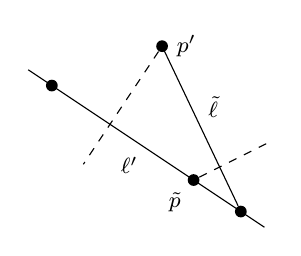
\begin{tikzpicture}
                \footnotesize
                \draw (0,2) -- node(p1)[pos=0.1,fill,circle,inner sep=1.5pt]{} node[below left]{$\ell'$} node(ptilde)[pos=0.7,fill,circle,inner sep=1.5pt,label={below left:$\tilde{p}$}]{} node(p2)[pos=0.9,fill,circle,inner sep=1.5pt]{} (3,0);
                \draw (1.7,2.3) node(p')[fill,circle,inner sep=1.5pt,label={right:$p'$}]{} -- node[above right]{$\tilde{\ell}$} (p2);

                \draw [dashed] (p') -- ++(-1,-1.5);
                \draw [dashed] (ptilde) -- ++(1,0.5);
            \end{tikzpicture}
            \caption{Sylvester's Theorem.}
            \label{fig:SylvestersTheorem}
        \end{figure}
        Consider points $p_i$ and lines $\ell_j$. Think about $d(p_i,l_j)$. At least one of these values will be nonzero. Thus, since there's only a finite number of distances, there will be a minimum nonzero value. Suppose $p'$ and $\ell'$ minimize nonzero $d$.
    \end{proof}
\end{enumerate}




\end{document}